\حصہ{اعدادی تکمل}
ہم نے دیکھا کہ  \عددی{f(x)} کے الٹ تفرق \عددی{F(x)} کے کلیہ سے قطعی تکمل \عددی{\int_a^bf(x)\dif x} کی قیمت  \عددی{F(b)-F(a)} حاصل کی جا سکتی ہے۔ بعض اوقات الٹ تفرق معلوم کرنا مشکل ہوتا ہے بلکہ بعض تفاعل، مثلاً \عددی{\tfrac{\sin x}{x}} اور \عددی{\sqrt{1+x^4}} کے الٹ تفرق کو بنیادی تفاعل کی صورت میں لکھنا ممکن نہیں ہوتا ہے۔ ہم یہ نہیں کہہ رہے ہیں کہ \عددی{\tfrac{\sin x}{x}} اور \عددی{\sqrt{1+x^4}}  کے الٹ تفرق کے کلیات اب تک کوئی حاصل کرنے میں کامیاب نہیں ہوا بلکہ ہم کہہ رہے ہیں کہ یہ ثابت کیا گیا ہے کہ ان تفاعل کے الٹ تفرق کو بنیادی تفاعل کی صورت میں نہیں لکھا جا سکتا ہے۔ 

ہم جب بھی قطعی تکمل کی قیمت کو الٹ تفرق سے حاصل کرنے میں نا کام ہوں، ہم اعدادی تراکیب، مثلاً  قاعدہ ذوزنقہ یا قاعدہ سمسن  بروئے کار لاتے ہیں جن پر اس حصہ میں غور کیا جائے گا۔

\حصہ{قاعدہ ذوزنقہ}
جب کسی تفاعل جس کی قطعی تکمل کی قیمت درکار ہو کے متکمل \عددی{f} کا الٹ تفرق ہم دریافت نہ کر سکیں تب ہم تکمل کے وقفہ کی خانہ بندی کرتے ہوئے ہر ذیلی وقفہ پر \عددی{f} کو تخمیناً موزوں کثیر رکنی سے ظاہر کر کے ان کثیر رکنیوں کا تکمل لے کر تمام جوابات کا مجموعہ لیتے ہیں جو تکمل کی تخمینی قیمت کے برابر ہو گا۔ کسی بھی خانہ بندی کے لئے جتنی زیادہ درجے کے کثیر رکنی منتخب کی جائیں حاصل جواب اتنا زیادہ درست ہو گا۔ کسی بھی درجے کی کثیر رکنی کے لئے جتنی باریک خانہ بندی کی جائے حاصل جواب اتنا زیادہ درست ہو گا حتٰی کے ہم پور و پور خلل یا حذفی خلل اتنا بڑھ جائے کہ مزید باریک خانہ بندی سے حاصل جواب کی درستگی کم ہونا شروع ہو جائے۔

\begin{figure}
\centering
\begin{minipage}{0.45\textwidth}
\centering
\begin{tikzpicture}[font=\small,    declare function={f(\x)=\x/4-sin(deg(\x*0.925))/2-1;}]
\begin{axis}[clip=false,small,axis lines=middle,xmin=0,xmax=11,xlabel={$x$},ylabel={$y$},xlabel style={at={(current axis.right of origin)},anchor=west},ylabel style={at={(current axis.above origin)},anchor=south},ytick={\empty}, xtick={4,5,6,7,8}, 
            extra x ticks={2,3},
            extra x tick style={
                xticklabel style={yshift=0.5ex, anchor=south}
            },xticklabels={$x_2$,,,$x_{n-1}$,\rlap{$x_n=b$}}, extra x tick labels={\llap{$x_0=a$},$x_1$}]
\addplot[domain=2:8,samples=7,]{f(x)};
\addplot[domain=2:8,samples=7,fill=lgray,on layer=background]{f(x)} \closedcycle;
\addplot[domain=2:8,samples=7,ycomb]{f(x)};
\addplot[stealth-stealth] plot coordinates {(5,-0.15) (6,-0.15)}node[pos=0.5,below]{$h$};
\addplot[] plot coordinates {(5,-0.1) (5,-0.2)};
\addplot[] plot coordinates {(6,-0.1) (6,-0.2)};
\draw(axis cs:2,{f(2)})node[pin=-45:{$N_0(x_0,y_0)$}]{};
\draw(axis cs:3,{f(3)})node[pin=-45:{$N_1(x_1,y_1)$}]{};
\draw(axis cs:4,{f(4)})node[pin={[pin distance=0.15cm]135:{$N_2(x_2,y_2)$}}]{};
\draw(axis cs:8,{f(8)})node[pin=-30:{$N_n(x_n,y_n)$}]{};
\addplot[domain=1:9,smooth,on layer=foreground]{f(x)}node[above]{$y=f(x)$};
\end{axis}
\end{tikzpicture}
\caption{ذوزنقہ قاعدہ برائے اعدادی تکمل۔}
\label{شکل_تکمل_ذوزنقہ_قاعدہ}
\end{minipage}\hfill
\begin{minipage}{0.45\textwidth}
\centering
\begin{tikzpicture}[declare function={f(\x)=\x^2;}]
\begin{axis}[small,axis lines=middle,xlabel={$x$},ylabel={$y$},xtick={1,1.25,1.5,1.75,2},xticklabels={$1$,$\tfrac{5}{4}$,$\tfrac{6}{4}$,$\tfrac{7}{4}$,$2$},xmax=2.25,ytick={\empty},xlabel style={at={(current axis.right of origin)},anchor=west},ylabel style={at={(current axis.above origin)},anchor=south}]
\addplot[domain=0:2.1]{f(x)};
\addplot[domain=1:2,samples=5,ycomb]{f(x)};
\draw(axis cs:1,3)node[left]{$y=x^2$};
\draw(axis cs:1,{f(1)})node[left]{$N_0$};
\draw(axis cs:1.25,{f(1.25)})node[left]{$N_1$};
\draw(axis cs:1.5,{f(1.5)})node[left]{$N_2$};
\draw(axis cs:1.75,{f(1.75)})node[left]{$N_3$};
\draw(axis cs:2,{f(2)})node[left]{$N_4$};
\draw(axis cs:1.125,{f(1.125)/2})node[]{$\tfrac{25}{16}$};
\draw(axis cs:1.375,{f(1.375)/2})node[]{$\tfrac{36}{16}$};
\draw(axis cs:1.625,{f(1.625)/2})node[]{$\tfrac{49}{16}$};
\draw(axis cs:1.875,{f(1.875)/2})node[]{$4$};
\end{axis}
\end{tikzpicture}
\caption{ذوزنقہ قاعدہ تفاعل $y=x^2$ کا رقبہ کچھ زیادہ دیتا ہے۔}
\label{شکل_مثال_تکمل_ذوزنقہ_قاعدہ_الف}
\end{minipage}
\end{figure}
کم درجے کی کثیر رکنی سے بھی اچھے نتائج حاصل ہوتے ہیں بلکہ مستقیم قطعات (درجہ \عددی{1} کثیر رکنی) بھی بہترین تخمین دیتے ہیں پس ان کی تعداد کافی ہونی چاہیے۔ اس کی وجہ سمجھنے کے لئے فرض کریں ہم \عددی{f} کے وقفہ \عددی{[a,b]} کو \عددی{\Delta x=h=\tfrac{b-a}{n}} لمبائی کے \عددی{n} قطعات میں تقسیم کر کے منحنی پر مطابقتی نقطوں کو سیدھے قطعات سے جوڑتے ہیں (شکل \حوالہ{شکل_تکمل_ذوزنقہ_قاعدہ})۔لمبائی \عددی{\Delta x=h=\tfrac{b-a}{n}} کو \اصطلاح{لمبائی قدم}\فرہنگ{قدم!لمبائی}\حاشیہب{step size}\فرہنگ{step!size} کہتے ہیں جس کو یہاں \عددی{\Delta x} کی بجائے \عددی{h} سے ظاہر کیا جاتا ہے جبکہ \عددی{n} \اصطلاح{قدموں}\فرہنگ{قدم}\حاشیہب{steps}\فرہنگ{steps} کی تعداد ہے۔ذیلی وقفوں کے آخری نقطوں سے تقسیمی نقطوں تک انتصابی لکیریں کھینچنے سے متعدد  ذوزنقہ حاصل ہوتے  ہیں جو منحنی اور \عددی{x} محور کے بیچ خطہ کی تخمین ہوں گے۔ ہم ان ذوزنقہ کے رقبوں کا مجموعہ لیتے ہیں جہاں \عددی{x}محور سے اوپر رقبہ کو مثبت جبکہ اس سے نیچے رقبہ کو منفی تصور کیا جاتا ہے۔
\begin{align*}
T&=\frac{1}{2}(y_0+y_1)h+\frac{1}{2}(y_1+y_2)h+\cdots+\frac{1}{2}(y_{n-2}+y_{n-1})h+\frac{1}{2}(y_{n-1}+y_n)h\\
&=h(\frac{1}{2}y_0+y_1+y_2+\cdots+y_{n-1}+\frac{1}{2}y_n)\\
&=\frac{h}{2}(y_0+2y_1+2y_2+\cdots+2y_{n-1}+y_n)
\end{align*}
یہاں \عددی{y_0=f(a)} ، \عددی{y_1=f(x_1)}، \نقطے، \عددی{y_{n-1}=f(x_{n-1})} اور \عددی{y_n=f(x_n)} ہیں۔

\ابتدا{قاعدہ}\موٹا{ذوزنقہ قاعدہ}\\
تکمل \عددی{\int_a^bf(x)\dif x} کو تخمیناً درج ذیل سے ظاہر کیا جا سکتا ہے (جہاں \عددی{n} ذیلی وقفوں کی لمبائی قدم \عددی{h=\tfrac{b-a}{n}} ہے اور \عددی{y_k=f(x_k)} ہے)۔
\begin{align}\label{مساوات_تکمل_ذوزنقہ_قاعدہ}
T=\frac{h}{2}(y_0+2y_1+2y_2+\cdots+2y_{n-1}+y_n)
\end{align}
\انتہا{قاعدہ}
%===================

\ابتدا{مثال}\شناخت{مثال_تکمل_ذوزنقہ_قاعدہ_الف}
تکمل \عددی{\int_1^2x^2\dif x}کو ذوزنقہ قاعدہ سے \عددی{n=4} لے کر حل کریں۔ اصل رقبہ کے ساتھ موازنہ کریں۔

حل:\quad
ہم وقفہ \عددی{[1,2]} کو چار برابر ذیلی وقفوں میں تقسیم کرتے ہیں۔یوں ایک وقفہ کی لمبائی \عددی{h=\tfrac{2-1}{4}=\tfrac{1}{4}} ہو گی۔ ان ذیلی وقفوں کے آخری نقطوں پر تفاعل \عددی{y=x^2} کی قیمت  درج ذیل ہے۔
\begin{align*}
\begin{array}{cc}
x&y=x^2\\
\hline
1&1\\[0.75ex]
\frac{5}{4}&\frac{25}{16}\\[0.75ex]
\frac{6}{4}&\frac{36}{16}\\[0.75ex]
\frac{7}{4}&\frac{49}{16}\\[0.75ex]
2&4\\
\hline
\end{array}
\end{align*}
 اب \عددی{n=4} اور \عددی{h=\tfrac{1}{4}} لیتے ہوئے مساوات \حوالہ{مساوات_تکمل_ذوزنقہ_قاعدہ} استعمال کرتے ہیں۔
\begin{align*}
T&=\frac{h}{2}(y_0+2y_1+2y_2+2y_3+y_4)\\
&=\frac{1}{8}(1+2(\tfrac{25}{16})+2(\tfrac{36}{16})+2(\tfrac{49}{16})+4)=\frac{75}{32}\\
&=\num{2.34375}
\end{align*} 
تکمل کی اصل قیمت درج ذیل ہے۔
\begin{align*}
\int_1^2x^2\dif x=\left.\frac{x^3}{3}\right\vert_1^2=\frac{8}{3}-\frac{1}{3}=\frac{7}{3}=2.\bar{3}
\end{align*}
یہاں تخمینی قیمت اصل قیمت سے زیادہ ہے۔ درحقیقت تمام ذوزنقے مطابقتی خطہ میں کچھ زیادہ رقبہ گھیرتا ہے (شکل \حوالہ{شکل_مثال_تکمل_ذوزنقہ_قاعدہ_الف})۔
\انتہا{مثال}
%=========================

\جزوحصہء{ذوزنقہ تخمین میں قابو خلل}
مختلف تفاعل کے ترسیم کو دیکھ کر ایسا معلوم ہوتا ہے  کہ لمبائی قدم \عددی{h} کم کرنے سے چونکہ ذوزنقہ تفاعل پر بہتر بیٹھتا ہے لہٰذا ذوزنقہ تخمین میں خلل
\begin{align}\label{مساوات_تکمل_خلل_ذوزنقہ_تعریف}
E_T=\int_a^bf(x)\dif x-T
\end{align}
 کم ہو گی۔اعلٰی احصاء کا ایک مسئلہ کہتا ہے کہ اگر \عددی{f} کا دہرا تفرق استمراری ہو تب یقینی طور پر ایسا ہی ہو گا۔

\موٹا{ذوزنقہ قاعدہ میں اندازہ خلل}\\
اگر \عددی{f''} استمراری ہو اور \عددی{[a,b]} پر \عددی{\abs{f''}} کی قیمت کی بالائی حد بندی \عددی{M}  ہو تب درج ذیل ہو گا۔
\begin{align}\label{مساوات_تکمل_ذوزنقہ_قاعدہ_خلل_مطلق}
\abs{E_T}\le \frac{b-a}{12}h^2M
\end{align} 

اگرچہ نظریہ کہتا ہے کہ ہر صورت \عددی{M} کی کم ترین قیمت پائی جائے گے عموماً حقیقت میں یہ قیمت جاننا ممکن نہیں ہوتا ہے۔ ہم عام طور پر \عددی{M} کی بہتر سے بہتر اندازاً قیمت معلوم کر کے اسی سے \عددی{\abs{E_TM}} حاصل کرتے ہیں۔ اگرچہ ایسا کرنا اچھا نہیں لگتا ہے لیکن یہ طریقہ چلتا ہے۔  کسی بھی \عددی{M} کے لئے \عددی{\abs{E_T}} کی قیمت کم کرنے کی خاطر ہم \عددی{h} کو چھوٹا کرتے ہیں۔ 

\ابتدا{مثال}
تکمل \عددی{\int_1^2x^2\dif x} کی تخمینی قیمت مثال \حوالہ{مثال_تکمل_ذوزنقہ_قاعدہ_الف} میں حاصل کی گئی۔ اس تخمینی قیمت میں خلل کی بالائی حد بندی تلاش کریں۔

حل:\quad
وقفہ \عددی{1\le x\le 2} پر \عددی{f(x)=x^2} کا دہرا تفرق \عددی{f''(x)=2} ہے جس کی قیمت اٹل ہے لہٰذا ہم \عددی{M=2} لے سکتے ہیں۔اب \عددی{b-a=1} اور \عددی{h=\tfrac{1}{4}} سے مساوات \حوالہ{مساوات_تکمل_ذوزنقہ_قاعدہ_خلل_مطلق} درج ذیل دیتی ہے۔ 
\begin{align*}
\abs{E_T}\le \frac{b-a}{12}h^2M=\frac{1}{12}\big(\frac{1}{4}\big)^2(2)=\frac{1}{96}
\end{align*}
ہم \عددی{\int_1^2x^2\dif x=\tfrac{7}{3}} سے \عددی{T=\tfrac{75}{32}} منفی کر کے یہی خلل
 \عددی{\abs{\tfrac{7}{3}-\tfrac{75}{32}}=\abs{-\tfrac{1}{96}}} حاصل کرتے ہیں۔ یہاں ہم خلل کی بالکل درست مطلق قیمت حاصل کرنے میں کامیاب ہوئے ہیں۔ ایسا ہر بار نہیں ہو گا۔
\انتہا{مثال}
%====================
\ابتدا{مثال}\شناخت{مثال_تکمل_خلل_درکار}
ذوزنقہ قاعدہ میں \عددی{n=10} قدم لیتے ہوئے درج ذیل تکمل کی تخمینی قیمت تلاش کریں (شکل \حوالہ{شکل_مثال_تکمل_خلل_درکار})۔
\begin{align*}
\int_0^{\pi}x\sin x\dif x
\end{align*}
%
\begin{figure}
\centering
\begin{tikzpicture}[declare function={f(\x)=\x*sin(deg(\x));}]
\begin{axis}[small,axis lines=middle,xtick={3.142},xticklabels={$\pi$},ytick={1,2},xmax=4,ymax=2.25,xlabel={$x$},ylabel={$y$}]
\addplot[domain=0:3.142,smooth]{f(x)}node[pos=0.5,left]{$y=x\sin x$};
\end{axis}
\end{tikzpicture}
\caption{متکمل برائے مثال \حوالہ{مثال_تکمل_خلل_درکار}}
\label{شکل_مثال_تکمل_خلل_درکار}
\end{figure}
حل:\quad
\عددی{a=0}، \عددی{b=\pi} اور \عددی{h=\tfrac{\pi-0}{10}} سے
\begin{align*}
\abs{E_T}\le \frac{b-a}{12}h^2M=\frac{\pi}{12}\big(\frac{\pi}{10}\big)^2M=\frac{\pi^3}{1200}M
\end{align*}
ملتا ہے جہاں \عددی{[0,\pi]} پر \عددی{f(x)=x\sin x} کے دہرا تفرق کی کوئی بھی بالائی حد بندی ہو سکتی ہے۔چونکہ
\begin{align*}
f''(x)=2\cos x-x\sin x
\end{align*}
کے برابر ہے لہٰذا درج ذیل ہو گا۔
\begin{align*}
\abs{f''(x)}&=\abs{2\cos x-x\sin x}\\
&\le 2\abs{\cos x}+\abs{x}\abs{\sin x}&&\text{\RL{تکونی عدم مساوات $\abs{a+b}\le \abs{a}+\abs{b}$}}\\
&\le 2\cdot 1+\pi\cdot 1=2+\pi&&\text{\RL{$\abs{\sin x}$ اور $\abs{\cos x}$ ایک سے بڑھ نہیں سکتے ہیں}}
\end{align*}
ہم \عددی{M=2+\pi} لیتے ہیں۔ یوں
\begin{align*}
\abs{E_T}\le \frac{\pi^3}{1200}M=\frac{\pi^3(2+\pi)}{1200}<0.133 &&\text{\RL{بطور حفاظت اوپر کو پورا کیا گیا ہے}}
\end{align*}
حاصل ہوتا ہے لہٰذا خلل کسی صورت بھی \عددی{0.133} سے زیادہ نہیں ہو گا۔ زیادہ درست جواب حاصل کرنے کی خاطر ہم \عددی{M} کی بہتر قیمت تلاش کرنے کی بجائے زیادہ قدم لیں گے، مثلاً \عددی{n=100} قدم لیتے ہوئے \عددی{h=\tfrac{1\pi}{100}} ہو گا جس سے خلل کم ہو کر درج ذیل رہ جاتا ہے۔
\begin{align*}
\abs{E_T}\le \frac{\pi}{12}\big(\frac{\pi}{100}\big)^2M=\frac{\pi^3(2+\pi)}{\num{120000}}<\num{0.00133}=1.33\times 10^{-3}
\end{align*}
\انتہا{مثال}
%====================
\ابتدا{مثال}
جیسا ہم باب میں دیکھیں گے \عددی{\ln 2} کی قیمت درج ذیل تکمل سے حاصل کی جا سکتی ہے۔
\begin{align*}
\ln 2=\int_1^2\frac{1}{x}\dif x
\end{align*}
ذوزنقہ قاعدہ سے تکمل کی قیمت حاصل کرتے ہوئے خلل کو \عددی{10^{-4}} سے کم رکھنے کی خاطر ہمیں کتنے قدم منتخب کرنے ہوں گے۔

حل:\quad
قدموں کی تعداد \عددی{n} یعنی ذیلی وقفوں کی تعداد منتخب کرنے کی خاطر ہم مساوات \حوالہ{مساوات_تکمل_ذوزنقہ_قاعدہ_خلل_مطلق} بروئے کار لاتے ہیں۔یوں
\begin{align*}
b-a=2-1=1,\quad h=\frac{b-a}{n}=\frac{1}{n},\quad f''(x)=\frac{\dif^{\,2}}{\dif x^2}(x^{-1})=2x^{-3}=\frac{2}{x^3}
\end{align*} 
سے  
\begin{align*}
\abs{E_T}\le \frac{b-a}{12}h^2\abs{f''(x)}_{\text{بلندتر}}=\frac{1}{2}\big(\frac{1}{n}\big)^2\abs{\frac{2}{x^3}}_{\text{بلندتر}}
\end{align*}
لکھا جا سکتا ہے جہاں وقفہ \عددی{[1,2]} پر \عددی{\abs{f''}_{\text{بلندتر}}} درکار ہے۔ 

یہ وہ شاذونادر موقع ہے جب ہم \عددی{\abs{f''}_{\text{بلندتر}}} کی ٹھیک ٹھیک قیمت معلوم کر سکتے ہیں۔ وقفہ \عددی{[1,2]} پر
 \عددی{y=\tfrac{2}{x^3}}  کی قیمت \عددی{y=2} سے گھٹ کر \عددی{y=\tfrac{1}{4}} ہوتی ہے۔یوں 
\begin{align*}
\abs{E_T}\le \frac{1}{12}\big(\frac{1}{n}\big)^2\cdot 2=\frac{1}{6n^2}
\end{align*}
ہو گا لہٰذا خلل کی مطلق قیمت  \عددی{10^{-3}} سے تب کم ہو گی جب \عددی{\frac{1}{6n^2}<10^{-4}} ہو جس سے درج ذیل حاصل ہو گا۔
\begin{align*}
\frac{1}{6n^2}&<10^{-4}\\
\frac{10^4}{6}&<n^2&&\text{\RL{دونوں اطراف کو $10^4n^2$ سے ضرب کریں}}\\
\frac{100}{\sqrt{6}}&<\abs{n}&&\text{\RL{جذر لیں}}\\
\frac{100}{\sqrt{6}}&<n&&\text{\RL{$n$ مثبت ہے}}\\
40.83&<n&&\text{\RL{حفاظتی طور پر اور کو پورا کیا گیا ہے۔}}
\end{align*}
عدد \عددی{40.83} سے بڑا پہلا عدد صحیح \عددی{41} ہے۔ یوں \عددی{n=41} یا اس سے بھی زیادہ  ذیلی وقفے لیتے ہوئے ذوزنقہ ترکیب سے \عددی{\ln 2} کی قیمت میں خلل کو یقینی طور پر  \عددی{10^{-4}} سے کم رکھا جا سکتا ہے۔ 
\انتہا{مثال}
%=====================

\جزوحصہء{سمسن قاعدہ}
قاعدہ سمسن میں \عددی{\int_a^bf(x)\dif x} کے حصول میں \عددی{f} کو مستقیم خطوط کی بجائے دو رتبی کثیر رکنی سے ظاہر کیا جاتا ہے۔ہم ترسیم کو سیدھی لکیروں کی بجائے قطع مکافی قوسین سے ظاہر کرتے ہیں۔ 

رتبی کثیر رکنی \عددی{y=Ax^2+Bx+C} کا \عددی{x=-h} تا \عددی{x=h} تکمل درج ذیل ہو گا۔
\begin{align*}
\int_{-h}^h(Ax^2+Bx+C)\dif x&=\left[\frac{Ax^3}{3}+\frac{Bx^2}{2}+Cx\right]_{-h}^h\\
&=\frac{2Ah^3}{3}+2Ch\\
&=\frac{h}{3}(2Ah^2+6C)
\end{align*}
کثیر رکنی کی مساوات سے 
\begin{align*}
y_0&=Ah^2-Bh+C,\quad y_1=C,\quad y_2=Ah^2+Bh+C
\end{align*}
لکھے جا سکتے ہیں جن سے درج ذیل حاصل ہوتے ہیں۔
\begin{align*}
C&=y_1\\
Ah^2-Bh&=y_0-y_1\\
Ah^2+Bh&=y_2-y_1\\
2Ah^2&=y_0+y_2-2y_1
\end{align*}
یوں حاصل تکمل میں \عددی{C} اور \عددی{2Ah^2} کی قیمتیں پر کرتے ہوئے
\begin{align*}
\frac{h}{3}(2Ah^2+6C)=\frac{h}{3}[(y_0+y_2-2y_1)+6y_1]=\frac{h}{3}(y_0+4y_1+y_2)
\end{align*}
یعنی
\begin{align}\label{مساوات_تکمل_قاعدہ_سمسن_الف}
\int_{-h}^hf(Ax^2+Bx+C)\dif x=\frac{h}{3}(y_0+4y_1+y_2)
\end{align}
ملتا ہے۔ وقفہ \عددی{[a,b]} کو برابر لمبائی کی جفت تعداد کی ذیلی وقفوں میں میں تقسیم کرتے ہوئے  مساوات \حوالہ{مساوات_تکمل_قاعدہ_سمسن_الف} کو یک بعد دیگرے ذیلی وقفوں کی جوڑیوں پر لاگو کر کے ان کا مجموعہ لینے سے  قاعدہ سمسن حاصل ہو گا۔

\موٹا{قاعدہ سمسن}\\
تکمل \عددی{\int_a^bf(x)\dif x} کا تخمین حاصل کرنے کے لئے درج ذیل استعمال کریں جو  \اصطلاح{قاعدہ سمسن}\فرہنگ{سمسن!قاعدہ}\حاشیہب{Simpson's rule}\فرہنگ{Simpson!rule} کہلاتا ہے۔ 
\begin{align}\label{مساوات_تکمل_قاعدہ_سمسن}
S&=\frac{h}{3}(y_0+4y_1+2y_2+4y_3+\cdots+2y_{n-2}+4y_{n-1}+y_n)
\end{align}
\عددی{y} کی قیمتیں نقطہ خانہ بندی
\begin{align*}
x_0=a,\, x_1=a+h,\, x_2=a+2h, \cdots, \, x_{n-1}=a+(n-1)h,\, x_n=b
\end{align*} 
پر لیے جاتے ہیں جہاں \عددی{n} جفت اور \عددی{h=\tfrac{b-a}{n}} ہے۔

\جزوجزوحصہء{قاعدہ سمسن میں قابو خلل}
قاعدہ سمسن میں خلل کی مقدار
\begin{align}\label{مساوات_تکمل_قاعدہ_سمسن_خلل_تعریف}
E_S=\int_a^bf(x)\dif x-S
\end{align} 
لمبائی قدم گھٹانے سے کم ہوتی ہے (جیسا قاعدہ ذوزنقہ بھی ہوتا ہے)  البتہ قاعدہ سمسن میں خلل قابو کرنے کے لئے درکار عدم مساوات میں \عددی{f} کے چار بار تفرق کا  استمراری ہونا ضروری ہے۔ اس بار بھی قابو خلل کا کلیہ اعلٰی احصاء دیتی ہے:

\موٹا{قاعدہ سمسن میں اندازاً خلل}\\
اگر \عددی{[a,b]} میں \عددی{f^{(4)}} استمراری ہو اور \عددی{\abs{f^{(4)}}} کی بالائی حد بندی کی کوئی ایک قیمت \عددی{M} ہو تب  مطلق خلل درج ذیل ہو گی۔
\begin{align}\label{مساوات_تکمل_قاعدہ_سمسن_خلل}
\abs{E_S}\le \frac{b-a}{180}h^4M
\end{align}

قاعدہ ذوزنقہ کی طرح ہم یہاں بھی عموماً \عددی{M} کی کم سے کم قیمت دریافت نہیں کر پائیں گے۔ ہم \عددی{M} کی کوئی موزوں قیمت تلاش کر کے اسی کو استعمال کرتے ہوئے \عددی{\abs{E_S}} کی تخمینی قیمت حاصل کرتے ہیں۔

\ابتدا{مثال}
درج ذیل تکمل کو قاعدہ سمسن سے حل کرتے ہوئے \عددی{n=4} لیں۔
\begin{align*}
\int_0^1 5x^4\dif x
\end{align*}
اس تخمین میں مساوات \حوالہ{مساوات_تکمل_قاعدہ_سمسن_خلل} کے تحت خلل اندازاً کتنی ہو گی؟

حل:\quad
ہم وقفہ تکمل کو چار برابر ذیلی وقفوں میں تقسیم کر کے تقسیمی نقطوں پر متکمل \عددی{f(x)=5x^4} کی قیمتیں حاصل کرتے ہیں۔
\begin{align*}
\renewcommand{\arraystretch}{1.5} 
\begin{array}{c|ccccc}
x&0&\frac{1}{4}&\frac{2}{4}&\frac{3}{4}&1\\
\midrule
f(x)&0&\frac{5}{256}&\frac{80}{256}&\frac{405}{256}&5
\end{array}
\end{align*}
ہم \عددی{n=4} اور \عددی{h=\tfrac{1}{4}} لیتے ہوئے مساوات \حوالہ{مساوات_تکمل_قاعدہ_سمسن} استعمال کرتے ہیں۔
\begin{align*}
S&=\frac{h}{3}(y_0+4y_1+2y_2+4y_3+y_4)\\
&=\frac{1}{12}\big[0+4\big(\frac{5}{256}\big)+2\big(\frac{80}{256}\big)+4\big(\frac{405}{256}\big)+5\big]\approx \num{1.00260}
\end{align*}
خلل جاننے سے پہلے ہمیں وقفہ \عددی{0\le x\le 1} پر  \عددی{f(x)=5x^4} کے چار بار تفرق \عددی{f^{(4)}} کی بالائی حد بندی کی ایک قیمت \عددی{M} چاہیے۔ چونکہ \عددی{f^{(4)}(x)=120} مستقل ہے لہٰذا ہم بلا خطر \عددی{M=120} لے سکتے ہیں۔ یوں \عددی{b-a=1} اور \عددی{h=\tfrac{1}{4}} استعمال کرتے ہوئے مساوات \حوالہ{مساوات_تکمل_قاعدہ_سمسن_خلل} سے درج ذیل حاصل ہوتا ہے۔
\begin{align*}
\abs{E_S}\le\frac{b-1}{180}h^4M=\frac{1}{180}\big(\frac{1}{4}\big)^4(120)=\frac{1}{384}<\num{0.00261} 
\end{align*}

\انتہا{مثال}
%========================
\جزوجزوحصہء{کونسا قاعدہ بہتر نتائج دیتا ہے؟}
قابو خلل کے کلیات 
\begin{align*}
\abs{E_T}\le \frac{b-1}{12}h^2M,\quad \abs{E_S}\le \frac{b-a}{180}h^4M
\end{align*}
سے یہ جانا جا سکتا ہے کہ کونسا کلیہ بہتر نتیجہ دیگا جہاں بائیں ہاتھ کلیہ میں \عددی{M}سے مراد \عددی{\abs{f''}} کی بالائی حد بندی ہے جبکہ دائیں ہاتھ کلیہ میں \عددی{M} سے مراد \عددی{\abs{f^{(4)}}} کی بالائی حد بندی ہے۔ اس کے علاوہ قاعدہ سمسن میں جزو  \عددی{\tfrac{b-a}{180}} قاعدہ ذوزنقہ میں جزو \عددی{\tfrac{b-a}{12}} سے \عددی{15} گنّا کم ہے۔ مزید قاعدہ سمسن میں \عددی{h^4} جبکہ قاعدہ ذوزنقہ میں \عددی{h^2} استعمال ہوتا ہے۔ یوں اگر \عددی{h=\tfrac{1}{10}} ہو تب \عددی{h^2=\tfrac{1}{100}} جبکہ \عددی{h^4=\tfrac{1}{10000}} ہو گا۔ اس طرح اگر دونوں \عددی{M} کی قیمت \عددی{1} اور  \عددی{b-a=1} ہوں تب \عددی{h=\tfrac{1}{10}} کی صورت میں  درج ذیل ہوں گے۔
\begin{align*}
\abs{E_T}&\le \frac{1}{12}\big(\frac{1}{10}\big)^2\cdot 1=\frac{1}{1200}\\
\abs{E_S}&\le \frac{1}{180}\big(\frac{1}{10}\big)^4\cdot 1=\frac{1}{\num{1800000}}=\frac{1}{1500}\cdot \frac{1}{1200}
\end{align*}
ایک جتنی حسابی کوشش سے اس مثال میں  قاعدہ سمسن بہت بہتر نتیجہ دیتا ہے۔

\عددی{h^4} بالمقابل \عددی{h^2} وہ اجزاء ہیں جن پر نظر رکھنی چاہیے۔ اگر \عددی{h} کی قیمت \عددی{1} سے کم ہو تب \عددی{h^4} کی قیمت \عددی{h^2} سے بہت کم ہو گی۔ اگر \عددی{h} کی قیمت \عددی{1} ہو تب \عددی{h^4=h^2} ہو گا۔ اگر \عددی{h} کی قیمت \عددی{1} سے زیادہ ہو تب \عددی{h^4} کی قیمت \عددی{h^2} سے بہت زیادہ ہو گی۔ ان آخری دو صورتوں میں قابو خلل کلیات  ہمیں زیادہ مدد فراہم نہیں کر سکتے ہیں اور ہمیں \عددی{y=f(x)} کی منحنی کو دیکھ کر فیصلہ کرنا ہو گا کہ  قاعدہ سمسن اور قاعدہ ذوزنقہ میں سے کونسا قاعدہ بہتر نتیجہ (اگر دیتا ہو) دیگا۔

\جزوجزوحصہء{اعدادی مواد کے ساتھ کام}
تجربہ گاہ میں پیمائش سے حاصل قیمتوں کو استعمال کرتے ہوئے قاعدہ سمسن کے ذریعہ ایسے تفاعل کے تکمل کی قیمت کو اگلے مثال میں حاصل کیا جائے گا جس کا کلیہ ہم  نہیں جانتے ہیں۔ ہم قاعدہ ذوزنقہ کو بھی اسی طرح  استعمال کر سکتے ہیں۔

\ابتدا{مثال}\شناخت{مثال_تکمل_گندے_پانی_کا_تالاب}
ایک شہر میں گندے پانی کا تالاب پایا جاتا ہے جس کو بھرنا مقصود ہے۔یہ تالاب \عددی{\SI{2.5}{\meter}} گہرا ہے (شکل \حوالہ{شکل_مثال_تکمل_گندے_پانی_کا_تالاب})۔ تالاب سے پانی کی نکاسی کرنے کے بعد اس کو مٹی سے بھرا جائے گا۔ کتنی مٹی درکار ہو گی؟ 

حل:\quad
تالاب کا حجم جاننے کے لئے ہم اس کا سطحی رقبہ کو \عددی{2.5} سے ضرب دیں گے۔ سطحی رقبہ کو قاعدہ سمسن سے حاصل کرتے ہیں جہاں \عددی{h=\SI{6}{\meter}} ہے جبکہ \عددی{y} کی قیمتوں کو تالاب پر ناپا گیا ہے (شکل \حوالہ{شکل_مثال_تکمل_گندے_پانی_کا_تالاب})۔
\begin{align*}
S&=\frac{h}{3}(y_0+4y_1+2y_2+4y_3+2y_4+4y_5+y_6)\\
&=\frac{6}{3}(30+100+40+100+36+40+7)=706
\end{align*}
سطحی رقبہ کو \عددی{2.5} سے ضرب دیتے ہوئے تقریباً \عددی{\SI{1765}{\meter\cubed}} حجم حاصل ہوتا ہے۔
\انتہا{مثال}
\begin{figure}
\centering
\begin{tikzpicture}
\begin{scope}
\clip(0,-0.2)rectangle (6,3.1);
\fill[smooth,lgray]  plot coordinates {(0,0)(1,0.1)(2,0.2)(3,0.5)(4,0.5)(5,0.2)(6,0)(6,0.7)(5,1.2)(4,2.3)(3,3)(2,2.2)(1,2.6)(0,3) (0,0)};
\end{scope}
\draw[smooth]  plot coordinates {(0,0)(1,0.1)(2,0.2)(3,0.5)(4,0.5)(5,0.2)(6,0)(6,0.7)(5,1.2)(4,2.3)(3,3)(2,2.2)(1,2.6)(0,3) (0,0)};
\path(0,0)--++(0,3)node[pos=0.5,sloped,above]{$\SI{30}{\meter}$};
\draw(1,0.1)--++(0,2.5)node[pos=0.5,sloped,above]{$\SI{25}{\meter}$};
\draw(2,0.2)--++(0,2)node[pos=0.5,sloped,above]{$\SI{20}{\meter}$};
\draw(3,0.5)--++(0,2.5)node[pos=0.5,sloped,above]{$\SI{25}{\meter}$};
\draw(4,0.5)--++(0,1.8)node[pos=0.5,sloped,above]{$\SI{18}{\meter}$};
\draw(5,0.2)--++(0,1)node[pos=0.5,sloped,above]{$\SI{10}{\meter}$};
\draw(6,0)--++(0,0.7)node[pos=0.5,sloped,above]{$\SI{7}{\meter}$};
\draw(6,0.35)++(0.04,0)--++(45:0.5cm)node[right]{\RL{نظر انداز}};
\draw[stealth-stealth](2,-0.1)--++(1,0)node[pos=0.5,below]{$\SI{6}{\meter}$};
\draw(2,0)--++(0,-0.2);
\draw(3,0)--++(0,-0.2);
\end{tikzpicture}
\caption{گندے پانی کا تالاب۔ افقی فاصلے $\SI{6}{\meter}$ ہیں (مثال \حوالہ{مثال_تکمل_گندے_پانی_کا_تالاب})۔}
\label{شکل_مثال_تکمل_گندے_پانی_کا_تالاب}
\end{figure}
%=========================

\جزوجزوحصہء{پور و پور خلل}
اگرچہ لمبائی قدم \عددی{h} کم کرنے سے ہم توقع کرتے ہیں کہ قاعدہ ذوزنقہ اور قاعدہ سمسن میں خلل کی مقدار کم ہو گی، حقیقت میں بعض اوقات اس کے برعکس بھی ہوتا ہے۔جب \عددی{h} کی قیمت بہت کم ہو، مثلاً \عددی{h=10^{-5}}، تب \عددی{S} اور \عددی{T} کی حساب میں پور و پور خلل اتنا بڑھ سکتا ہے کہ نتائج میں بہتری کی بجائے خرابی پیدا ہو سکتی ہے۔ایسی صورت میں آپ کلیات خلل، جو پور و پور خلل کو جاننے سے قاصر ہیں، پر بھروسہ نہیں کر سکتے ہیں۔ لمبائی قدم \عددی{h} کو کسی خاص قیمت سے کم کرنے سے حقیقتاً نتائج خراب ہو سکتے ہیں۔ اس کتاب میں ایسی صورت حال پیدا نہیں ہو گی۔ اگر آپ کو ایسی صورت حال کا سامنا ہو، بہتر ہو گا کہ آپ اعدادی تراکیب پر لکھی گئی کسی کتاب کا سہارا لیں۔

\حصہء{سوالات}
\موٹا{تکمل کی قیمت کا اندازہ}\\
سوال \حوالہ{سوال_تکمل_اندازہ_ذوزنقہ_سمسن_الف} تا سوال \حوالہ{سوال_تکمل_اندازہ_ذوزنقہ_سمسن_ب} میں دو جزو پائے جاتے ہیں۔ایک جزو قاعدہ ذوزنقہ اور دوسرا جزو قاعدہ سمسن کے  لئے ہے۔
\begin{enumerate}[1.]
\item
قاعدہ ذوزنقہ
\begin{enumerate}[a.]
\item
چار قدم \عددی{n=4} لے کر تکمل کی تخمینی قیمت تلاش کریں۔ مساوات \حوالہ{مساوات_تکمل_ذوزنقہ_قاعدہ_خلل_مطلق} سے خلل \عددی{\abs{E_T}} کی بالائی حدود بندی کی قیمت دریافت کریں۔
\item
تکمل کو حل کرتے ہوئے مساوات \حوالہ{مساوات_تکمل_خلل_ذوزنقہ_تعریف} سے \عددی{\abs{E_T}} تلاش کریں۔
\item
خلل \عددی{\abs{E_T}} کو اصل تکمل  کے فی صد کی صورت میں لکھیں۔
\end{enumerate}
\item
قاعدہ سمسن
\begin{enumerate}[a.]
\item
چار قدم \عددی{n=4} لے کر تکمل کی تخمینی قیمت تلاش کریں۔ مساوات \حوالہ{مساوات_تکمل_قاعدہ_سمسن_خلل}  سے خلل \عددی{\abs{E_S}} کی بالائی حدود بندی کی قیمت دریافت کریں۔
\item
تکمل کو حل کرتے ہوئے مساوات \حوالہ{مساوات_تکمل_قاعدہ_سمسن_خلل_تعریف} سے \عددی{\abs{E_S}} تلاش کریں۔
\item
خلل \عددی{\abs{E_S}} کو اصل تکمل  کے فی صد کی صورت میں لکھیں۔
\end{enumerate}
\end{enumerate}

\ابتدا{سوال}\شناخت{سوال_تکمل_اندازہ_ذوزنقہ_سمسن_الف}
$\int_1^2x\dif x$
\انتہا{سوال}
%========================
\ابتدا{سوال}
$\int_1^3(2x-1)\dif x$
\انتہا{سوال}
%========================
\ابتدا{سوال}
$\int_{-1}^{1}(x^2+1)\dif x$
\انتہا{سوال}
%========================
\ابتدا{سوال}
$\int_{-2}^{0}(x^2-1)\dif x$
\انتہا{سوال}
%========================
\ابتدا{سوال}
$\int_{0}^{2}(t^3+t)\dif t$
\انتہا{سوال}
%========================
\ابتدا{سوال}
$\int_{-1}^{1}(t^3+1)\dif t$
\انتہا{سوال}
%========================
\ابتدا{سوال}
$\int_{1}^{2}\tfrac{1}{s^2}\dif s$
\انتہا{سوال}
%========================
\ابتدا{سوال}\شناخت{سوال_تکمل_اندازہ_ذوزنقہ_سمسن_پ}
$\int_{2}^{4}\tfrac{1}{(s-1)^2}\dif s$
\انتہا{سوال}
%========================
\ابتدا{سوال}
$\int_{0}^{\pi}\sin t\dif t$
\انتہا{سوال}
%========================
\ابتدا{سوال}\شناخت{سوال_تکمل_اندازہ_ذوزنقہ_سمسن_ب}
$\int_{0}^{1}\sin \pi t\dif t$
\انتہا{سوال}
%========================
سوال \حوالہ{سوال_تکمل_جدول_الف} تا سوال \حوالہ{سوال_تکمل_جدول_ب} میں (ا) قاعدہ ذوزنقہ، (ب) قاعدہ سمسن استعمال کرتے ہوئے دی گئی قیمتیں استعمال کرتے ہوئے آٹھ قدم \عددی{n=8} کے لئے تکمل حل کریں۔ اپنے جواب کو \عددی{5} اعشاریہ درستگی تک پور و پور کریں۔ (ج) اس کے بعد تکمل کی اصل قیمت حاصل کریں اور خلل \عددی{\abs{E_T}}  کو مساوات \حوالہ{مساوات_تکمل_خلل_ذوزنقہ_تعریف} اور خلل \عددی{\abs{E_S}} کو مساوات \حوالہ{مساوات_تکمل_قاعدہ_سمسن_خلل_تعریف} سے حاصل کریں۔

\ابتدا{سوال}\شناخت{سوال_تکمل_جدول_الف}
$\int_0^1 x\sqrt{1-x^2}\dif x$
\begin{align*}
\begin{array}{>{\scriptstyle}c|*9{>{\scriptstyle}l}}
x&0&0.125&0.25&0.375&0.5&0.625&0.75&0.875&1.0\\
\midrule
x\sqrt{1-x^2}&0.0&0.12402&0.24206&0.34763&0.43301&0.48789&0.49608&0.42361&0
\end{array}
\end{align*}
\انتہا{سوال}
%=====================
\ابتدا{سوال}
$\int_0^3 \tfrac{\theta}{\sqrt{16+\theta^2}}\dif \theta$
\begin{align*}
\begin{array}{>{\scriptstyle}c|*9{>{\scriptstyle}l}}
\theta&0&0.375&0.75&1.125&1.5&1.875&2.25&2.625&3.0\\
\midrule
\tfrac{\theta}{\sqrt{16+\theta^2}}&0.0&0.09334&0.18429&0.27075&0.35112&0.42443&0.49026&0.58466&0.6
\end{array}
\end{align*}
\انتہا{سوال}
%=====================
\ابتدا{سوال}
$\int_{-\pi/2}^{\pi/2} \tfrac{3\cos t}{(2+\sin t)^2}\dif t$
\begin{align*}
\begin{array}{>{\scriptstyle}c|*9{>{\scriptstyle}c}}
t&-1.5708&-1.1781&-0.7854&-0.3927&0&0.3927&0.7854&1.1781&1.5708\\
\midrule
\tfrac{3\cos t}{(2+\sin t)^2}&0.0&0.99138&1.26906&1.05961&0.75&0.48821&0.28946&0.13429&0
\end{array}
\end{align*}
\انتہا{سوال}
%=====================
\ابتدا{سوال}\شناخت{سوال_تکمل_جدول_ب}
$\int_{\pi/4}^{\pi/2} (\csc^2y)\sqrt{\cot y}\dif y$
\begin{align*}
\begin{array}{>{\scriptstyle}c|*9{>{\scriptstyle}c}}
y&0.78540&0.88357&0.98175&1.07992&1.17810&1.27627&1.37445&1.47262&1.57080\\
\midrule
(\csc^2y)\sqrt{\cot y}&2.0&1.51606&1.18237&0.93998&0.75402&0.60145&0.46364&0.31688&0
\end{array}
\end{align*}
\انتہا{سوال}
%=====================
\موٹا{ذیلی وقفوں کی کم سے کم تعداد}\\
سوال \حوالہ{سوال_تکمل_ذیلی_وقفوں_کی_تعداد_الف} تا سوال \حوالہ{سوال_تکمل_ذیلی_وقفوں_کی_تعداد_ب} میں خلل کی مقدار \عددی{10^{-4}} سے کم مطلوب ہے۔ (ا) قاعدہ ذوزنقہ اور (ب) قاعدہ سمسن استعمال کریں۔  مساوات \حوالہ{مساوات_تکمل_ذوزنقہ_قاعدہ_خلل_مطلق} اور مساوات \حوالہ{مساوات_تکمل_قاعدہ_سمسن_خلل} کی مدد سے ذیلی وقفوں کی درکار تعداد تلاش کریں۔ (سوال \حوالہ{سوال_تکمل_ذیلی_وقفوں_کی_تعداد_الف} تا سوال \حوالہ{سوال_تکمل_ذیلی_وقفوں_کی_تعداد_پ} درحقیقت سوال \حوالہ{سوال_تکمل_اندازہ_ذوزنقہ_سمسن_الف} تا سوال \حوالہ{سوال_تکمل_اندازہ_ذوزنقہ_سمسن_پ} ہیں۔) 

\ابتدا{سوال}\شناخت{سوال_تکمل_ذیلی_وقفوں_کی_تعداد_الف}
$\int_1^2x\dif x$
\انتہا{سوال}
%========================
\ابتدا{سوال}
$\int_1^3(2x-1)\dif x$
\انتہا{سوال}
%========================
\ابتدا{سوال}
$\int_{-1}^1(x^2+1)\dif x$
\انتہا{سوال}
%========================
\ابتدا{سوال}
$\int_{-2}^0(x^2-1)\dif x$
\انتہا{سوال}
%========================
\ابتدا{سوال}
$\int_0^2(t^3+t)\dif t$
\انتہا{سوال}
%========================
\ابتدا{سوال}
$\int_{-1}^1(t^3+1)\dif t$
\انتہا{سوال}
%========================
\ابتدا{سوال}
$\int_1^2\tfrac{1}{s^2}\dif s$
\انتہا{سوال}
%========================
\ابتدا{سوال}\شناخت{سوال_تکمل_ذیلی_وقفوں_کی_تعداد_پ}
$\int_2^4\tfrac{1}{(s-1)^2}\dif s$
\انتہا{سوال}
%========================
\ابتدا{سوال}
$\int_0^3\sqrt{x+1}\dif x$
\انتہا{سوال}
%========================
\ابتدا{سوال}
$\int_0^3\tfrac{1}{\sqrt{x+1}}\dif x$
\انتہا{سوال}
%========================
\ابتدا{سوال}
$\int_0^2\sin(x+1)\dif x$
\انتہا{سوال}
%========================
\ابتدا{سوال}\شناخت{سوال_تکمل_ذیلی_وقفوں_کی_تعداد_ب}
$\int_{-1}^1\cos(x+\pi)\dif x$
\انتہا{سوال}
%========================
\موٹا{عملی استعمال}\\
\ابتدا{سوال}\شناخت{سوال_تکمل_تالاب_مچھلی}
آپ کے شہر میں ایک جھیل ہے جس کی اوسط گہرائی \عددی{\SI{7}{\meter}} ہے جبکہ اس کا سطحی رقبہ شکل \حوالہ{شکل_سوال_تکمل_تالاب_مچھلی} میں دکھایا گیا ہے۔ ماہی گیری کے موسم کی شروع میں اوسطاً فی \عددی{\SI{9}{\meter\cubed}} ایک مچھلی پائی جاتی ہے۔ماہی گیری کے ایک اجازت نامہ پر اوسطاً فی موسم \عددی{20} مچھلیاں شکار کی جاتی ہیں۔ موسم کے اختتام پر جھیل میں پہلے دن کے لحاظ سے \عددی{\SI{25}{\percent}} مچھلی باقی رہنا ضروری ہے۔  ماہی گیری کے موسم میں کتنے اجازت  نامے منظور کیے جا سکتے ہیں؟ ترکیب سمسن استعمال کریں۔  
\begin{figure}
\centering
\begin{tikzpicture}[x=0.75cm,y=0.75cm,font=\small]
\draw[fill=lgray] plot[smooth cycle] coordinates {(0,0) (1,-1.7) (2,-2.3) (3,-2.6) (4,-2.5) (5,-2.2) (6,-1.4) (7,-0.8) (8,0) (7,0.9) (6,1.1) (5,1.2)(4,1.5)(3,1.7) (2,1.8) (1,1.5)};
\draw(1,-1.7)--(1,1.5)node[pos=0.5,sloped,below]{$\SI{320}{\meter}$};
\draw(2,-2.3)--(2,1.8)node[pos=0.5,sloped,below]{$\SI{410}{\meter}$};
\draw(3,-2.6)--(3,1.7)node[pos=0.5,sloped,below]{$\SI{430}{\meter}$};
\draw(4,-2.5)--(4,1.5)node[pos=0.5,sloped,below]{$\SI{400}{\meter}$};
\draw(5,-2.2)--(5,1.2)node[pos=0.5,sloped,below]{$\SI{340}{\meter}$};
\draw(6,-1.4)--(6,1.1)node[pos=0.5,sloped,below]{$\SI{250}{\meter}$};
\draw(7,-0.8)--(7,0.9)node[pos=0.5,sloped,below]{$\SI{170}{\meter}$};
\draw(0,0)node[rotate=90,below]{$\SI{0}{\meter}$};
\draw(8,0)node[rotate=90,below]{$\SI{0}{\meter}$};
\draw[stealth-stealth](3,-2.8)--++(1,0)node[pos=0.5,below]{$\SI{70}{\meter}$};
\draw(3,-2.7)--++(0,-0.2);
\draw(4,-2.7)--++(0,-0.2);
\end{tikzpicture}
\caption{جھیل برائے سوال \حوالہ{سوال_تکمل_تالاب_مچھلی}}
\label{شکل_سوال_تکمل_تالاب_مچھلی}
\end{figure}

جواب:\quad \عددی{4873}
\انتہا{سوال}
%=====================
\ابتدا{سوال}\شناخت{سوال_تکمل_ہوائی_پر}
جہاز کا \اصطلاح{ہوائی پترا}\فرہنگ{ہوائی پترا}\حاشیہب{aerofoil}\فرہنگ{aerofoil} شکل \حوالہ{شکل_سوال_تکمل_ہوائی_پر} میں دکھایا گیا ہے جس میں \عددی{\SI{25000}{\liter}} تیل کی ٹینکی واضح ہے۔ تیل کی کثافت \عددی{\SI{0.708}{\kilo\gram\per\liter}} ہے۔ درج ذیل معلومات دی گئی ہیں جن کے بیچ افقی فاصلہ \عددی{\SI{30}{\centi\meter}} ہے۔تیل کی ٹینکی کی لمبائی تلاش کریں۔
\begin{align*}
y_0=\SI{45}{\centi\meter},\,y_1=\SI{48}{\centi\meter},\,y_2=\SI{54}{\centi\meter},\,y_3=\SI{57}{\centi\meter},\,y_4=\SI{60}{\centi\meter},\,y_5=y_6=\SI{63}{\centi\meter}
\end{align*}
\begin{figure}
\centering
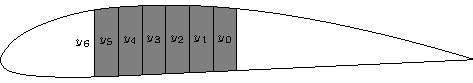
\includegraphics{airfoilClark}
\caption{ہوائی پترا}
\label{شکل_سوال_تکمل_ہوائی_پر}
\end{figure}

\انتہا{سوال}
%=======================
\ابتدا{سوال}\شناخت{سوال_تکمل_شمسی_گاڑی}
شمسی چادر سے حاصل برقی طاقت سے چلنے والی گاڑی کا رقبہ عمودی تراش شکل \حوالہ{شکل_سوال_تکمل_شمسی_گاڑی} میں دکھایا گیا ہے۔ہوائی مزاحمت کا کچھ حصہ رقبہ عمودی تراش پر منحصر ہوتا ہے لہٰذا کوشش کی جاتی ہے کہ رقبہ عمودی تراش کو کم سے کم رکھا جائے۔ اس گاڑی کا رقبہ عمودی تراش قاعدہ سمسن سے دریافت کریں۔ 

جواب:\quad \عددی{\SI{2973}{\centi\meter\squared}}
\begin{figure}
\centering
\begin{tikzpicture}[scale=0.5,font=\scriptsize]
\draw[name path=seat] plot [smooth cycle] coordinates {(0,0)(1,-0.75)(2,-1.2)(3,-1.4)(4,-1.2)(5,-0.75)(6,0) (5,1.8)(4,2.28) (3,2.46) (2,2.28) (1,1.8)};
\draw(1,-0.75)--(1,1.8)node[pos=0.5,sloped,above]{$\SI{48}{\centi\meter}$};
\draw(2,-1.2)--(2,2.28)node[pos=0.5,sloped,above]{$\SI{61}{\centi\meter}$};
\draw(3,-1.4)--(3,2.46)node[pos=0.5,sloped,above]{$\SI{66}{\centi\meter}$};
\draw(4,-1.2)--(4,2.28)node[pos=0.5,sloped,above]{$\SI{61}{\centi\meter}$};
\draw(5,-0.75)--(5,1.8)node[pos=0.5,sloped,above]{$\SI{48}{\centi\meter}$};
\draw(0,-0.5)--++(0,-1.2);
\draw(6,-0.5)--++(0,-1.2);
\draw[stealth-stealth](0,-1.6)--++(6,0)node[pos=0.5,below]{$\SI{60}{\centi\meter}$};
\draw[name path=lwheel]([shift={(0:0.25cm and 2cm)}]-2,0) arc (0:360:0.25cm and 2cm)coordinate[pos=0.15](kA)coordinate[pos=0.9](kB)node[pos=0.4,pin=135:{پہیا}]{};
\draw[name path=rwheel]([shift={(0:0.25cm and 2cm)}]8,0) arc (0:360:0.25cm and 2cm)coordinate[pos=0.35](kAA)coordinate[pos=0.6](kBB);
\path[name path=uL](kA)--++(3,0);
\path[name path=uLD](kA)--++(-40:3);
\path[name path=uLL](kB)--++(4,0);
\draw[name intersections={of=uL and seat}](kA)--(intersection-1);
\draw[name intersections={of=uLD and seat}](kA)--(intersection-1);
\draw[name intersections={of=uLL and seat}](kB)--(intersection-1);
%
\path[name path=uL](kAA)--++(-3,0);
\path[name path=uLD](kAA)--++(-140:3);
\path[name path=uLL](kBB)--++(-4,0);
\draw[name intersections={of=uL and seat}](kAA)--(intersection-1);
\draw[name intersections={of=uLD and seat}](kAA)--(intersection-1);
\draw[name intersections={of=uLL and seat}](kBB)--(intersection-1);
\end{tikzpicture}
\caption{شمسی گاڑی برائے سوال \حوالہ{سوال_تکمل_شمسی_گاڑی}}
\label{شکل_سوال_تکمل_شمسی_گاڑی}
\end{figure}
\انتہا{سوال}
%========================
\ابتدا{سوال}
ایک گاڑی ساکن حالت سے روانہ ہو کر \عددی{\SI{130}{\kilo\meter\per\hour}} تک \عددی{\SI{37.1}{\second}} میں پہنچ پاتی ہے۔ اس کی رفتار بالمقابل وقت درج ذیل ہے۔
\begin{align*}
\begin{array}{c|cccc cccc cccc}
\si{\kilo\meter\per\hour}&0&30&40&50&60&70&80&90&100&110&120&130\\
\midrule
\si{\second}&0&2.2&3.2&4.5&5.9&7.8&10.2&12.7&16&20.6&26.2&37.1
\end{array}
\end{align*}
اس رفتار تک پہنچتے ہوئے گاڑی کتنا فاصلہ طے کرتی ہے؟
\انتہا{سوال}
%============================
\موٹا{نظریہ اور مثالیں}\\
\ابتدا{سوال}\ترچھا{کم درجی کثیر رکنیاں}\\
تکمل \عددی{\int_a^bf(x)\dif x} میں خلل
\begin{align*}
\abs{E_T}=\frac{b-a}{12}h^2\abs{f''(c)}
\end{align*}
ہے جہاں  وقفہ \عددی{[a,b]} میں \عددی{c} (عموماً نا معلوم) نقطہ ہے۔ اگر \عددی{f} متغیر \عددی{x} کا خطی تفاعل ہو تب \عددی{f''(c)=0}  لہٰذا \عددی{E_T=0} ہو گا اور کسی بھی \عددی{h} کے لئے تکمل کی اصل قیمت \عددی{T} ہو گی۔ یہ تعجب کی بات نہیں ہے چونکہ خطی تفاعل کی صورت میں ترسیم کو تخمینی طور پر ظاہر کرنے والے قطعات ترسیم پر ٹھیک بیٹھیں گے۔  تعجب کی بات سمسن خلل
\begin{align*}
\abs{E_S}=\frac{b-a}{180}h^4\abs{f^{(4)}(c)}
\end{align*} 
ہے جو درجہ چار سے کم کثیر رکنی  \عددی{f}  کی صورت میں ہر \عددی{c} کے لئے  \عددی{f^{(4)}(c)=0} کی بنا \عددی{E_S=0} ہو گا اور یوں اگر ہم صرف دو قدم بھی استعمال کریں تب بھی \عددی{S} تکمل کی اصل قیمت ہو گی۔یہ دیکھنے کی خاطر \عددی{n=2} لیتے ہوئے درج ذیل کی اندازاً قیمت قاعدہ سمسن سے  تلاش کر کے تکمل کی اصل قیمت کے ساتھ موازنہ کریں۔
\begin{align*}
\int_0^2x^3\dif x
\end{align*}
\انتہا{سوال}
%=======================
\ابتدا{سوال}\شناخت{سوال_تکمل_سائن_تکمل}\ترچھا{تفاعل سائن تکمل کی قابل استعمال قیمتیں}\\
تفاعل سائن تکمل
\begin{align*}
\kSi(x)=\int_0^x\frac{\sin t}{t}\dif t\quad\quad\text{\RL{$x$ کا سائن تکمل}}
\end{align*}
ان تفاعل میں سے ایک ہے جنہیں بنیادی تفاعل کی صورت میں لکھنا ممکن نہیں ہے۔ تفاعل \عددی{\tfrac{\sin t}{t}} کے الٹ تفرق کا کلیہ نہیں پایا جاتا ہے البتہ اعدادی تراکیب سے \عددی{\kSi(x)} کی قیمتیں با آسانی حاصل کی جا سکتی ہیں۔ 

اگرچہ تکمل سائن لکھتے ہوئے یہ حقیقت بظاہر نظر نہیں آتی ہے درحقیقت ہم درج ذیل تفاعل کا تکمل حاصل کرنا چاہتے ہیں
\begin{align*}
f(t)=
\begin{cases}
\frac{\sin t}{t},&t\ne 0\\
1,&t=0
\end{cases}
\end{align*}
جو \عددی{\tfrac{\sin t}{t}} کی وقفہ \عددی{[0,x]} تک  استمراری توسیع ہے۔ اس تفاعل کی دائرہ کار کے ہر نقطہ پر تفاعل کے ہر رتبہ کے تفرق پائے جاتے ہیں۔ اس کا ترسیم ہموار ہے (شکل \حوالہ{شکل_سوال_تکمل_سائن_تکمل}) اور ہم قاعدہ سمسن سے بہترین نتائج توقع کرتے ہیں۔
\begin{enumerate}[a.]
\item
وقفہ \عددی{[0,\pi/2]} پر \عددی{\abs{f^{(4)}}\le 1} ہے۔اس حقیقت کو استعمال کرتے ہوئے \عددی{n=4} لیتے ہوئے درج ذیل کو قاعدہ سمسن سے حاصل کرتے ہوئے خلل کی بالائی حد بندی تلاش کریں۔
\begin{align*}
\kSi\big(\frac{\pi}{2}\big)=\int_0^{\pi/2}\frac{\sin t}{t}\dif t
\end{align*}
\item
\عددی{n=4} لیتے ہوئے قاعدہ سمسن سے \عددی{\kSi(\pi/2)} حاصل کریں۔
\item
جزو-ا میں خلل کو جزو-ب میں قیمت کا فی صد لکھیں۔
\end{enumerate}
\انتہا{سوال}
%=========================
\begin{figure}
\centering
\begin{tikzpicture}[declare function={f(\x)=sin(deg(\x))/\x;},font=\small]
\begin{axis}[axis on top,clip=false,small,axis lines=middle,xtick={-3.142,3.142,6.284,2},xticklabels={$-\pi$,$\pi$,$2\pi$,$x$},ytick={\empty},xlabel={$t$},ylabel={$y$},ymax=1.25,xlabel style={at={(current axis.right of origin)},anchor=west}]
\addplot[domain=-4:7,smooth]{f(x)};
\draw(axis cs:2,{f(2)})--(2,0);
\addplot[name path=ksin,domain=0:2,draw=none,smooth]{f(x)};
\draw[name path=axis](axis cs:0,0)--(axis cs:2,0);
\addplot[fill=lgray]fill between [of=axis and ksin];
\draw(axis cs:1,{3/4*f(1)})node[pin=45:{$\kSi(x)=\int\limits_0^x\frac{\sin t}{t}\dif t$}]{};
\draw(axis cs:-1,{f(-1)})node[left]{$y=\frac{\sin t}{t}$};
\end{axis}
\end{tikzpicture}
\caption{تفاعل سائن تکمل (سوال \حوالہ{سوال_تکمل_سائن_تکمل})}
\label{شکل_سوال_تکمل_سائن_تکمل}
\end{figure}
\ابتدا{سوال}
خلل کی حد بندی مساوات \حوالہ{مساوات_تکمل_ذوزنقہ_قاعدہ_خلل_مطلق} اور مساوات \حوالہ{مساوات_تکمل_قاعدہ_سمسن_خلل} دیتی ہیں۔ حقیقت میں قاعدہ ذوزنقہ اور قاعدہ سمسن کے نتائج اس سے بہتر ہوں گے۔ مثال \حوالہ{مثال_تکمل_خلل_درکار} میں \عددی{\int_0^{\pi}x\sin x\dif x} کی اندازاً قیمت کو قاعدہ ذوزنقہ سے حاصل کیا گیا۔
\begin{enumerate}[a.]
\item
قاعدہ ذوزنقہ میں \عددی{n=10} لیتے ہوئے تکمل کو دوبارہ حل کریں۔
\item
تکمل کی اصل قیمت \عددی{\pi} اور آپ کے حاصل کردہ جواب میں فرق دریافت کریں۔ آپ دیکھیں گے کہ  مثال \حوالہ{مثال_تکمل_خلل_درکار} میں \عددی{n=10}کے لئے حاصل خلل \عددی{0.133} سے موجودہ خلل بہت کم ہے۔
\item
ہم  \عددی{[0,\pi]} پر \عددی{\abs{f''(x)}=\abs{2\cos x-x\sin x}}کی بہتر حد بندی معلوم کر کے  مثال \حوالہ{مثال_تکمل_خلل_درکار} میں \عددی{\abs{E_T}} کی بالائی حد بندی کو \عددی{0.133} سے بہتر بنا سکتے ہیں۔ \عددی{\abs{f''(x)}} کو کمپیوٹر پر ترسیم کر کے مطلوبہ خطہ کو بڑا کرتے ہوئے بہتر بالائی حد بندی دریافت کر کے اس کو بطور \عددی{M} لے کر \عددی{\abs{E_T}}کی بہتر قیمت تلاش کریں۔ آپ دیکھیں گے کہ جزو-ا میں حاصل نتیجہ اس سے بھی بہتر ہو ہے۔
\end{enumerate}
\انتہا{سوال}
%====================
\ابتدا{سوال}
\begin{enumerate}[a.]
\item
دکھائیں کہ \عددی{f(x)=x\sin x} کا چار بار تفرق \عددی{f^{(4)}=-4\cos x+x\sin x} ہے۔ کمپیوٹر پر اس کو وقفہ \عددی{[0,\pi]} پر ترسیم کر کے مطلوبہ خطہ کو بڑا کر کے اس کی بالائی حد بندی دیکھ کر دریافت کریں۔
\item
جزو-ا میں حاصل قیمت کو \عددی{M} لے کر قاعدہ سمسن میں \عددی{n=10} لیتے ہوئے  درج ذیل تکمل حاصل کرنے میں خلل کی بالائی حد بندی  کو  مساوات \حوالہ{مساوات_تکمل_قاعدہ_سمسن_خلل} سے حاصل کریں۔
\begin{align*}
\int_0^{\pi}x\sin x\dif x
\end{align*}
\item
قاعدہ سمسن میں \عددی{n=10} لے کر \عددی{\int_0^{\pi}x\sin x\dif x} کی قیمت حاصل کریں۔
\item
تکمل کی اصل قیمت \عددی{\pi} اور جزو-ج میں حاصل جواب میں فرق کو \عددی{6} اعشاریہ درستگی تک لکھیں۔ آپ دیکھیں گے کہ جزو-ب میں حاصل خلل کافی درست ہے۔
\end{enumerate}
\انتہا{سوال}
%===================
